\subsection{Исполнение и контроль проекта. Затраты по фазам проекта}

Исполнение и контроль проекта --- часто эти процессы ставят рядом и считают их родственными.
Эти процессы действительно тесно взаи­мосвязаны, однако координация проекта --- это не контроль.
Несмотря на то что процессы координации содержат некоторые элементы конт­роля, для обеспечения полноценного и эффективного мониторинга работ, своевременного выявления отклонений от плановых показателей менеджер проекта выстраивает систему контроля своего проекта.

Контроль --- сравнение фактического исполнения с запланированным, анализ отклонений, оценка тенденций для оказания влияния на улучшение процесса, оценка альтернатив и рекомендация корректирующих действий, если это не­обходимо.

Процессы мониторинга и контроля --- процессы, выполняемые в целях из­мерения и мониторинга исполнения проекта, чтобы в случае необходимости можно было прибегнуть к корректирующим действиям для управления исполнением фазы или проекта.

Анализ и регулирование выполнения проекта --- стадия процесса управ­ления проектом, на которой осуществляются: сравнение фактического выпол­нения с запланированным, анализ отклонений, прогноз их влияния на конеч­ные результаты и оценка возможных корректирующих действий \cite[190--191]{polkovnikov}.

Обычно вследствие непредсказуемых изменений внешнего окружения проекта и непредвиденных внутренних обстоятельств длительность выполнения проекта и фактическая стоимость отличаются от запланированных.
Кроме того, с течением времени могут измениться и потребности, для удовлетворения которых разрабатывался проект.
Внесение изменений является обычным явлением в любом проекте.
Первоначальный план может оказаться несостоятельным из-за различных факторов, например из-за сдвига сроков начала проекта, пересмотра условий финансирования, изменения потребностей, неточного планирования связей между задачами, временных оценок и ресурсных требований задач, срыва поставок документации или оборудования подрядчиками, неожиданных технических затруднений и изменения внешних условий.
Однако многие отклонения от плана могут быть сглажены своевременным и эффективным руководством.

Таким образом, все основные элементы проекта должны контролироваться руководством.
Менеджер должен определить процедуру и установить последовательность сбора данных через определенные интервалы времени, производить анализ полученных данных, анализировать текущие расхождения фактических и плановых показателей и прогнозировать влияние текущего состояния дел на выполнение оставшихся объемов работ.

Требования к системе контроля, включающие состав анализируемой информации, структуру отчетов и ответственность за сбор данных, анализ информации и принятие решений, вырабатываются до начала реализации проекта с участием всех заинтересованных сторон.
Система руководства проектом должна обеспечивать корректирующие воздействия там и тогда, где и когда они необходимы.
Например, если происходит задержка окончания отдельных работ, то, возможно, ускорить их выполнение можно за счет перераспределения трудовых ресурсов и оборудования.
Если же задерживается поставка проектной документации, увеличиваются затраты на материалы и оборудование, субподрядчики срывают директивные сроки, то необходимо пересмотреть план проекта.
Коррекция плана может быть ограничена пересмотром параметров задач, а может потребовать разработки совершенно новой сетевой модели, начиная с текущего состояния и до момента окончания проекта.

Основные принципы построения эффективной системы контроля включают:

Наличие четких планов.
Планы должны быть содержательны, четко структурированы и фиксированы, с тем чтобы обеспечивать основу для контроля.
Если планы обновляются слишком часто и без применения процедур контроля за изменениями, контроль над проектом может быть потерян.

Наличие ясной системы отчетности.
Отчеты должны отображать состояние проекта относительно исходных планов на основании единых подходов и критериев.

Процедуры подготовки и получения отчетов должны быть четко определены и достаточно просты.
Четкие временные интервалы должны быть определены для всех видов отчетов.

Результаты, представленные в отчетах, должны обсуждаться на совещаниях.

Наличие эффективной системы анализа фактических показателей и тенденций.
В результате анализа собранных данных руководство проекта должно определить, соответствует ли текущая ситуация запланированной, а если нет, то рассчитать размер и серьезность последствий отклонений.
Двумя основными показателями прогресса являются время и стоимость.
Специальные отчеты должны использоваться для предсказания тенденций в стоимостных и временных оценках работ проекта.
В наиболее простом случае предсказания могут указывать на увеличение стоимости проекта или задержки по срокам.
Однако часто отклонения во временных и стоимостных показателях оказывают также влияние на содержание предстоящих работ и качество результатов.


Наличие эффективной системы реагирования.
Завершающим шагом процесса контроля являются действия, предпринимаемые руководством и направленные на преодоление отклонений в ходе работ проекта.
Эти действия могут быть направлены на исправление выявленных недостатков и преодоление негативных тенденций в рамках проекта.
Однако в ряде случаев может потребоваться пересмотр плана.
Перепланирование требует проведения анализа «Что, если...», обеспечивающего предсказание и расчет последствий от планируемых действий.
От менеджера зависит также убеждение и мотивация команды проекта в необходимости тех или иных действий.

Процесс контроля проекта
В рамках функции контроля и оперативного управления реализацией проекта решаются задачи измерения, прогнозирования и оценки складывающейся оперативной ситуации по достижению результатов, затратам времени, ресурсов и финансов, анализу и устранению причин отклонения от выработанного плана, коррекция плана.
Обычно при управлении проектом контролируются три основные количественные характеристики --- время, объем работ и стоимость.
Кроме того, руководство отвечает за управление содержанием работ (изменениями), качеством и организационной структурой.

Важным для анализа хода работ параметром является текущая дата (пороговая дата), которая представляет собой как бы момент времени, относительно которого производится анализ.
Состояние работ по проекту оценивается относительно пороговой даты.

Основные методы анализа состояния работ, используемые менеджером, предусматривают сбор фактических данных о достигнутых результатах и оценку фактических затрат, оценку оставшегося объема работ, анализ фактической выработки на текущую дату.

Руководство должно установить последовательность сбора данных через определенные интервалы времени, производить анализ полученных данных, анализировать текущие расхождения фактических и плановых показателей и прогнозировать влияние текущего состояния дел на затраты по оставшемуся объему работ.

Таким образом, в процессе контроля можно выделить три основных шага:

\begin{enumerate}
	\item Отслеживание фактического состояния работ - сбор и документирование фактических данных.
	\item Анализ результатов и измерение прогресса - оценка текущего состояния работ и сравнение достигнутых результатов с запланированными;
	\item Корректирующие действия --- планирование и осуществление действий, направленных на выполнение работ в соответствии с планом или минимизацию несоответствий.
\end{enumerate}

Обобщенная схема процесса управления исполнением проекта представлена на рисунке \ref{fig:ris7}.
\begin{figure}[!h]
	\centering
	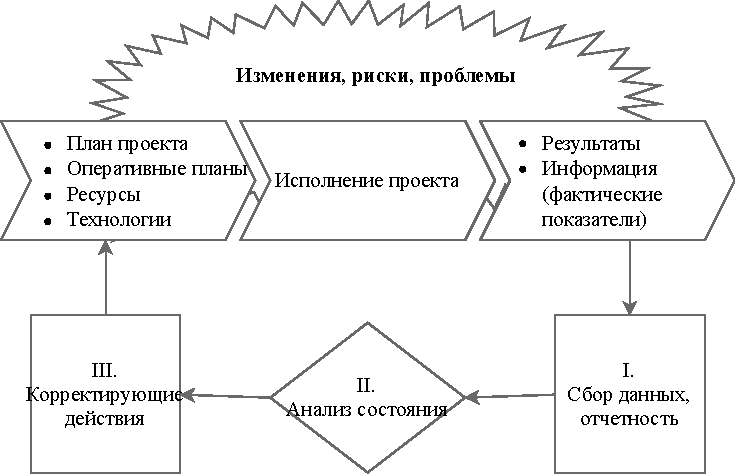
\includegraphics[width=\linewidth]{control}
	\caption{Обобщенная схема процесса контроля исполнения проекта}
	\label{fig:ris7}
\end{figure}
